\documentclass[xcolor=svgnames,t]{beamer} 
\usepackage[utf8]{inputenc}
\usepackage{booktabs, comment}
\usepackage{graphicx}  % Add graphicx package
\usepackage[absolute, overlay]{textpos} 
\usepackage{pgfpages}
\usepackage[font=footnotesize]{caption}
\useoutertheme{infolines} 
\usepackage{xcolor}
% \usepackage{cite}  % REMOVE this line because it conflicts with natbib
\usepackage{colortbl}
\definecolor{brownbrown}{RGB}{8, 8, 9}
\usepackage[round, sort, authoryear]{natbib}  % Use only natbib for citation management
\definecolor{brownred}{RGB}{198, 198, 198}

\setbeamercolor{title in head/foot}{bg=brownred, fg=brownbrown}
\setbeamercolor{author in head/foot}{bg=myuniversity}
\setbeamertemplate{page number in head/foot}{}

\usepackage{amsmath}
\usepackage[makeroom]{cancel}

\newtheorem{equi}{} %Creates a grey box when equi is called
\setbeamertemplate{navigation symbols}{} 
\usepackage{textpos}

\usepackage{tikz}

\usetheme{Madrid}
\definecolor{myuniversity}{RGB}{48, 67, 180}
\usecolortheme[named=myuniversity]{structure}
\usepackage{tikz}


\usepackage{colortbl} 
\newcommand{\myitem}{\item[$\circ$]}
\newcommand{\witem}{\item[\textcolor{white}{$\bullet$}]}
\DeclareMathOperator*{\argmax}{arg\,max}
\DeclareMathOperator*{\argmin}{arg\,min}
\AtBeginSection[]{
\begin{frame}
\frametitle{Content}
\tableofcontents[currentsection]
\end{frame}
}

\title[Introduction to Causal Inference]{Introduction to Causal Inference}
\subtitle{}
%\titlegraphic{\includegraphics[height=1cm]{brown-logo.png}}  % This line is commented out to remove the logo
\author[CIML ]{Causal Inference using Machine Learning\\ Master in Economics, UNT}
\institute[]{Andres Mena}
\date{Spring 2024}

\addtobeamertemplate{navigation symbols}{}{%
    \usebeamerfont{footline}%
    \usebeamercolor[fg]{footline}%
    \hspace{1em}%
    \insertframenumber/\inserttotalframenumber
}

\begin{document}
\begin{frame}
\maketitle
\end{frame}

%%%%%%%%%%%%%%%%%%%%%%%%%%%%
%\logo{\includegraphics[height=0.5cm]{brown-arms.png}}  % This line is commented out to remove the logo
%%%%%%%%%%%%%%%%%%%%%%%%%%

\begin{frame}
    \frametitle{Table of Contents}
    \tableofcontents
\end{frame}

\section{What is Causal Inference?}
\begin{frame}
    \frametitle{What is a Causal Question?}
    
    % Show the image first
    \begin{center}
    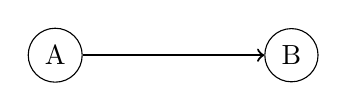
\begin{tikzpicture}
        \node[draw, circle] (A) at (0,0) {A};
        \node[draw, circle] (B) at (3,0) {B};
        \draw[->, thick] (A) -- (B);
    \end{tikzpicture}
    \end{center}
    
    \pause % Transition to the bullet points
    
    A causal question asks about the effect of a cause \(A\) on an outcome \(B\).
    
    \pause % Transition to the first main bullet
    \begin{itemize}
        \item \(A\) could be: % Introduce sub-bullets for A
        \begin{itemize}
            \pause
            \item Policy (e.g., a new transfer policy impacting household income (AUH))
            \pause
            \item Treatment (e.g., a drug trial reducing heart attack risk)
            \pause
            \item Business strategy (e.g., a marketing campaign affecting sales)
            \pause
            \item Technological innovation (e.g., the introduction of innovation of supply chain)
        \end{itemize}
        
        \pause % Transition to the second main bullet
        \item \(B\) could be: % Single item + example for B
        \begin{itemize}
            \pause
            \item Welfare (e.g., income, poverty, crime, happiness, inequality)
            \pause
            \item Health (e.g., life expectancy, disease risk, heart attacks)
            \pause
            \item Profits (e.g., company earnings,  market share, costs)
            \pause
            \item Efficiency (e.g., speed of production or resource utilization)
        \end{itemize}
    \end{itemize}
\end{frame}



\begin{frame}
    \frametitle{Correlation is not Causation (and vice versa)}

    \textbf{1. Correlation \(\cancel{\rightarrow}\) Causation}
    
    \pause % Transition to correlation definition
    
    \begin{itemize}
        \item \textbf{Correlation}: A statistical relationship between two variables, where changes in one variable are associated with changes in another. 
        \[
        \text{Corr}(A, B) = \frac{\text{Cov}(A, B)}{\sigma_A \sigma_B}
        \]
    \end{itemize}
    
    \pause % Transition to correlation example
    
    \begin{itemize}
        \item Example: Rain and umbrellas. 
    \end{itemize}

    \pause % Transition to the causation part

    \textbf{2. Causation \(\cancel{\rightarrow}\) Correlation}

    \pause % Transition to causation definition
    
    \begin{itemize}
        \item \textbf{Causation}: A direct effect of one variable on another, where \(A\) causes \(B\).
        \[
        B = f(A)
        \]
    \end{itemize}
    
    \pause % Transition to causation example
    
    \begin{itemize}
        \item Example: Eating more food can cause weight gain, but if food intake and exercise both increase proportionally, we may observe no correlation between food and weight in the data, even though causation exists.
    \end{itemize}

\end{frame}

\begin{frame}
    \frametitle{Causal Inference Tree}
    \begin{figure}
        \includegraphics[width=0.8\linewidth]{Figures/CI_tree.jpg}
        \caption{Source: Scott Cunningham Substack}
    \end{figure}
\end{frame}

\begin{frame}
    \frametitle{Experimental Design Tradition}
    
    Experimental design relies on randomized controlled trials (RCTs) to establish causality through direct manipulation of the treatment.

    \begin{itemize}
        \item \cite{neyman1923}: 
        \begin{itemize}
         \item Introduced the \textbf{potential outcomes} framework for randomized experiments.
        \end{itemize}
        
        \pause
        \item \cite{fisher1935}: 
        \begin{itemize}
            \item Random assignment removes selection bias.
        \end{itemize}
        
        \pause
        \item \cite{rubin1974}: 
        \begin{itemize}
            \item Generalized the potential outcomes framework to both observational and experimental studies.
        \end{itemize}
        
        \pause
        \item \cite{banerjee2011}: 
        \begin{itemize}
            \item Duflo and Banerjee pioneered the use of RCTs in development economics to evaluate the impact of poverty alleviation policies.
    \end{itemize}
    \end{itemize}
\end{frame}


\begin{frame}
    \frametitle{Quasi-experimental Design}
    
    \small % Reduce font size to fit the text
    Explodes natural variation and perform comparisons under identification assumptions.
    \pause
    \begin{itemize}
        \item \textbf{Difference-in-Differences (DiD)}: \cite{snow1854} used natural variation in water sources to compare cholera outcomes between neighborhoods. \\
            \hspace{10pt}-\textit{CQ}: Does contaminated water cause cholera?
        
        \pause % Transition to IV
        \item \textbf{Instrumental Variables (IV)}: \cite{wright1928} used exogenous supply-side instruments (rain) to estimate demand for agricultural products. \\
            \hspace{10pt}-\textit{CQ}: What is the effect of price on the quantity demanded?
        
        \pause % Transition to RD
        \item \textbf{Regression Discontinuity (RD)}: \cite{thistlethwaite1960} studied the effect of merit awards on student performance. \\
            \hspace{10pt}-\textit{CQ}: What is the effect of winning a merit award on future academic success?
        
        \pause % Transition to SCM
        \item \textbf{Synthetic Control (SCM)}: \cite{abadie2003}: developed SCM to run comparative case studies. \\
            \hspace{10pt}-\textit{CQ}: What is the impact of Terrorism on Economic Performance?
    \end{itemize}
\end{frame}

\begin{frame}
    \frametitle{Machine Learning and Causal Inference}

    \textbf{What is Machine Learning?}
    \begin{itemize}
        \item Machine Learning (ML) refers to algorithms and statistical models that allow computers to learn from and make predictions or decisions based on data.
        \item ML excels at identifying complex patterns and making predictions in high-dimensional settings.
    \end{itemize}

    \pause % Transition to causal inference

    \textbf{How Machine Learning is Used in Causal Inference}
    \begin{itemize}
        \item Machine Learning can be used to estimate nuisance parameters (e.g., propensity scores, regression functions) in causal inference models.
        \item \cite{chernozhukov2018double} introduced \textbf{Double/Debiased Machine Learning (DML)}, which combines machine learning for estimating high-dimensional nuisance functions with traditional econometric techniques to ensure valid causal inference.
        \item ML algorithms are employed in tasks like instrumental variable estimation, heterogeneous treatment effects, and controlling for high-dimensional confounders.
    \end{itemize}

    \pause % Mention DML's impact
    \begin{block}{Key Advantage of ML for Causal Inference}
        ML allows researchers to handle large datasets with many covariates while reducing the bias that arises from complex relationships between variables. 
    \end{block}

\end{frame}


\section{The Four Questions of Causal Inference}

\begin{frame}
    \frametitle{1. What's the Causal Relationship of Interest?}

    Causal inference begins by identifying the causal relationship of interest. Some classic papers are examples of the main methodologies:
    \begin{itemize}
        \item Difference-in-Differences (DiD): How do historical institutions impact modern economic development? \cite{acemoglu2001}
        
        \pause
        \item Instrumental Variables (IV): What is the causal effect of compulsory schooling on earnings? \cite{angrist1991education}
        
        \pause
        \item Comparative Case Study: How do immigration shocks affect local labor markets? \cite{card1990mariel}
    \end{itemize}

    These questions seek to determine the effect of specific treatments (institutions, education, immigration) on outcomes of interest (development, earnings, labor markets).
\end{frame}

\begin{frame}
    \frametitle{The Experimental Ideal}

    \textbf{What is the ideal experiment to capture the treatment/causal effect?}
    \pause
    \begin{itemize}
        \item The experimental ideal serves as a benchmark for understanding causal effects, helping to evaluate the identification strategy.
        \item \pause
        \item It is often an abstract or hypothetical experiment with no practical, ethical, or financial constraints.
        \item \pause
        \item Example: \cite{bauer2015} 
        \begin{itemize}
            \pause
            \item Research Question: What is the causal effect of victimization (being robbed) on social trust?
            \item \pause
            \item Ideal Experiment: 
            \begin{itemize}
                \pause
                \item Randomly sample individuals from the target population (e.g., Swiss population).
                \item \pause
                \item Homogeneous robbers administer the same factual negative experience to the treatment group, while others are left undisturbed (control group).
                \item \pause
                \item Measure trust levels directly before and after the treatment to control timing.
            \end{itemize}
        \end{itemize}
    \end{itemize}
    
    
\end{frame}


\begin{frame}
    \frametitle{3. What's the Identification Strategy?}

    Causal inference requires a strategy to identify the causal effect. The strategy relies on exogenous variability and assumptions:
    
    \begin{itemize}
        \pause
        \item \textbf{Instrumental Variables (IV)}: 
        \begin{itemize}
            \item Strategy: Use of instruments that affect the treatment but not the outcome directly (e.g., proximity to a college \cite{angrist1991education}).
            \item Assumption: \textbf{Exclusion Restriction}, \textbf{Relevance}.
        \end{itemize}

        \pause
        \item \textbf{Difference-in-Differences (DiD)}: 
        \begin{itemize}
            \item Strategy: Compare treated and control groups over time.
            \item Assumption: \textbf{Parallel Trends}.
        \end{itemize}

        \pause
        \item \textbf{Regression Discontinuity (RD)}: 
        \begin{itemize}
            \item Strategy: Use a cutoff or threshold to identify the causal effect.
            \item Assumption: \textbf{Local Randomization}, \textbf{Continuity of Potential Outcomes}.
        \end{itemize}
    \end{itemize}
\end{frame}

\begin{frame}
    \frametitle{4. What's the Inference Strategy?}

    After identifying the causal effect, we need to make valid statistical inferences. Common inference strategies include:
    \begin{itemize}
        \item \textbf{Delta Method}: 
        \begin{itemize}
            \item pproximate the variance (or standard error) of a function of an estimator, by using a first-order Taylor expansion.
        \end{itemize}

        \pause
        \item \textbf{Bootstrap}: 
        \begin{itemize}
            \item Re-sample the data multiple times to approximate the sampling distribution of an estimator. 
        \end{itemize}

        \pause
        \item \textbf{Influence Functions}: 
        \begin{itemize}
            \item Analyze the sensitivity of the estimator to small changes in the sample. Common in non-parametric estimation.
        \end{itemize}
    \end{itemize}

    Each strategy allows for valid inference under different circumstances, depending on the complexity of the model and data.
\end{frame}



\section{Probability Essentials}
\begin{frame}{Random Variable and Probability Measure}
    \textbf{Random Variable:}
    \begin{itemize}
      \item A random variable \( X \) is a measurable function from the sample space \( \Omega \) to the real numbers: 
      \[
      X: \Omega \rightarrow \mathbb{R}
      \]
    \end{itemize}

    \vspace{0.5cm}
    \pause
    \textbf{Probability Measure:}
    \begin{itemize}
        \item A probability measure \( P \) is a function that assigns a probability to each event \( A \in \mathcal{F} \), where \( \mathcal{F} \) is a sigma-algebra over the sample space \( \Omega \), such that:

    \end{itemize}
    \pause
    \vspace{0.5cm}
    \begin{enumerate}[<+->]
        \item \textbf{Non-negativity}: \( P(A) \geq 0 \) for any event \( A \in \mathcal{F} \).
        \item \textbf{Normalization}: \( P(\Omega) = 1 \).
        \item \textbf{Additivity}: For disjoint events \( A_1, A_2, \dots \), 
        \[
        P\left( \bigcup_{i=1}^{\infty} A_i \right) = \sum_{i=1}^{\infty} P(A_i)
        \]
    \end{enumerate}
\end{frame}

\begin{frame}{Binary Outcome and Sigma Algebra}
    \textbf{Binary Outcome and Probability Measure:}
    \begin{itemize}
      \item Define the sample space \( \Omega = \{High, Low\} \).
      \item The sigma-algebra \( \mathcal{F} \) is the power set of \( \Omega \), i.e.,
      \[
      \mathcal{F} = \{\emptyset, \{Low\}, \{High\}, \{Low, High\}\}
      \]
      \item Define \( Y \in \{High, Low\} \), with the following values and probabilities:
    \end{itemize}
    
    \vspace{0.3cm}
    \centering
    \begin{table}[]
        \begin{tabular}{|c|c|}
            \hline
            \( i \) & \( Y \) \\ \hline
            1 & Low  \\ \hline
            2 & Low  \\ \hline
            \rowcolor{blue!20} 3 & High \\ \hline
            \rowcolor{blue!20} 4 & High \\ \hline
            \rowcolor{blue!20} 5 & High \\ \hline
            \rowcolor{blue!20} 6 & High \\ \hline
            \end{tabular}
    \end{table}
    
    \small{
    \begin{itemize}
        \item \( P(Y = Low) = 0.33 \), \( P(Y = High) = 0.66 \)
    \end{itemize}
    }
\end{frame}

\begin{frame}{Verification of Probability Axioms}
    \textbf{Verification of Axioms:}
    \begin{enumerate}[<+->]
      \item \textbf{Non-negativity}: For all elements in \( \mathcal{F} \),
      \[
      P(\emptyset) = 0, \quad P(\{Low\}) = 0.33, \quad P(\{High\}) = 0.66, \quad P(\{Low, High\}) = 1
      \]
      All probabilities are non-negative.
      
      \item \textbf{Normalization}: The total probability of the sample space:
      \[
      P(\{Low, High\}) = P(Y = Low) + P(Y = High) = 0.33 + 0.66 = 1
      \]
      
      \item \textbf{Additivity}: For disjoint events in \( \mathcal{F} \),
      \[
      P(\{Low\} \cup \{High\}) = P(\{Low\}) + P(\{High\}) = 0.33 + 0.66 = 1
      \]
      \[
      P(\{Low\} \cup \emptyset) = P(\{Low\}) + P(\emptyset) = 0.33 + 0 = 0.33
      \]
      \[
      P(\{High\} \cup \emptyset) = P(\{High\}) + P(\emptyset) = 0.66 + 0 = 0.66
      \]
    \end{enumerate}
\end{frame}






\begin{frame}{Venn Diagram, Conditional Probability, and Independence}
  \begin{center}
    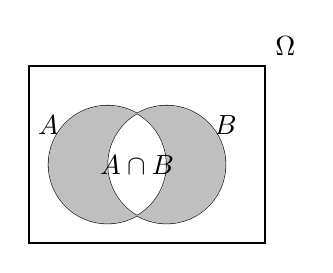
\begin{tikzpicture}[scale=0.5]
        % Draw a box around the Venn diagram representing the sample space \Sigma
        \draw[thick] (-2, -2) rectangle (4, 2.5) node[above right] {\(\Omega\)};
        
        % Draw the Venn diagram circles
        \draw (0,0) circle (1.5cm) node at (-1.5, 1) {\( A \)};
        \draw (1.5,0) circle (1.5cm) node at (3, 1) {\( B \)};
        
        % Draw the intersection and label it
        \fill[gray!50] (0,0) circle (1.5cm) [even odd rule] (1.5,0) circle (1.5cm);
        \node at (0.75, 0) {\( A \cap B \)};
    \end{tikzpicture}
    
  \end{center}
   

    \vspace{0.3cm}
    
    \textbf{Conditional Probability:}
    \begin{itemize}
      \item The conditional probability of \( A \) given \( B \) is defined as:
      \[
      P(A|B) = \frac{P(A \cap B)}{P(B)}, \quad \text{for } P(B) > 0
      \]
    \end{itemize}
    
    \vspace{0.3cm}

    \textbf{Independence:}
    \begin{itemize}
      \item Two events \( A \) and \( B \) are independent if:
      \[
      P(A \cap B) = P(A)P(B)
      \]
    \end{itemize}
\end{frame}
\begin{frame}{Exogenous D}
    \textbf{Binary Outcome with New Variable \( D \): \( D \sim \text{Bernoulli}(0.5) \)}
    
    \centering
    \begin{table}[]
    \begin{tabular}{|c|c|c|}
    \hline
    \( i \) & \( Y \) & \( D \) \\ \hline
    1 & Low  & 0 \\ \hline
    2 & Low  & 1 \\ \hline
    3 & Low  & 0 \\ \hline
    \rowcolor{blue!20} 4 & High & 1 \\ \hline
    5 & High & 0 \\ \hline
    6 & Low  & 1 \\ \hline
    \end{tabular}
    \end{table}

    \small{
    \begin{itemize}
      \item \( P(D = 1) = 0.5 \), \( P(Y = High) = 0.33 \)
      \item Joint probability: \( P(Y = High \cap D = 1) = \frac{1}{6} = 0.167 \)
      \item Independence check: 
      \[
      P(Y = High)P(D = 1) = 0.33 \times 0.5 = 0.165
      \]
      \item Independence check: 
      \[
      P(Y = High|P(D = 1) =   P(Y = High) = 0.33
      \]
    \end{itemize}
    }
\end{frame}



\begin{frame}{Endogenous Assignment of \( D \)}
    \textbf{Binary Outcome with Endogenous \( D \): \( D \sim \text{Bernoulli}(p(Y)) \), where \( p(Y^{High}) > p(Y^{Low}) \)}
    
    \centering
    \begin{table}[]
    \begin{tabular}{|c|c|c|}
    \hline
    \( i \) & \( Y \) & \( D \) \\ \hline
    1 & Low  & 0 \\ \hline
    \rowcolor{blue!20} 2 & High & 1 \\ \hline
    3 & Low  & 0 \\ \hline
    \rowcolor{blue!20} 4 & High & 1 \\ \hline
    5 & Low  & 1 \\ \hline
    6 & High & 0 \\ \hline
    \end{tabular}
    \end{table}

    \small{
    \begin{itemize}
      \item \( P(Y = High) = 0.5 \), \( P(D = 1) = 0.5 \)
      \item \item \( P(Y = High \cap D = 1) = 0.33 \neq 0.5 *0.5  \)
      \item \( P(Y = High | D = 1) = \frac{0.33}{0.5} = 0.67 = \frac{2}{3}\)
      
    \end{itemize}
    }
\end{frame}

\begin{frame}{Law of Total Probability}
    \textbf{Law of Total Probability:}
    \[
    P(Y = H) = P(Y = H | D = 1)P(D = 1) + P(Y = H | D = 0)P(D = 0)
    \]
    
    \vspace{0.5cm}
    Using the values from our example:
    \begin{itemize}
        \item \( P(Y = High | D = 1) = \frac{2}{3} = 0.67 \)
        \item \( P(D = 1) = 0.5 \)
        \item \( P(Y = High | D = 0) = \frac{1}{3} = 0.33 \)
        \item \( P(D = 0) = 0.5 \)
    \end{itemize}
    
    \vspace{0.5cm}
    Therefore, applying the law of total probability:
    \[
    P(Y = High) = 0.67 \times 0.5 + 0.33 \times 0.5 = 0.335 + 0.165 = 0.5
    \]
    
    \vspace{0.5cm}
    This matches the marginal probability \( P(Y = High) = 0.5 \) calculated earlier.
\end{frame}


\begin{frame}{Expectation }
    \begin{columns}
        % Column 1: Discrete Variable Expectation
        \begin{column}{0.45\textwidth}
            \textbf{Expectation (Discrete Variable):}
            \begin{itemize}
                \item For a discrete random variable \( X \) with probability mass function \( p(x) \):
                \[
                \mathbb{E}[X] = \sum_{x \in \mathcal{X}} x \cdot p(x)
                \]
                where \( \mathcal{X} \) is the set of possible values of \( X \).
            \end{itemize}
            \pause
            \vspace{0.3cm}
            
            \textbf{Example: Bernoulli(0,1)}
            \begin{itemize}
                \item \( X \in \{0,1\} \quad P(X = 1) = 0.5 \) 
                \item \( \mathbb{E}[X] = 1 \cdot 0.5 + 0 \cdot 0.5 = 0.5 \)
            \end{itemize}
        \end{column}
        
        \pause
        
        % Column 2: Continuous Variable Expectation
        \begin{column}{0.45\textwidth}
            \textbf{Expectation (Continuous Variable):}
            \begin{itemize}
                \item For a continuous random variable \( X \) with probability density function \( f(x) \):
                \[
                \mathbb{E}[X] = \int_{-\infty}^{\infty} x \cdot f(x) \, dx
                \]
                where \( f(x) \) is the PDF of \( X \).
            \end{itemize}
            
            \pause
            
            \vspace{0.3cm}
            
            \textbf{Example: Normal(0,1)}
            \begin{itemize}
                \item \( X \sim N(0, 1) \), where the PDF is \( f(x) = \frac{1}{\sqrt{2\pi}} e^{-x^2/2} \)
                \item \( \mathbb{E}[X] = \int_{-\infty}^{\infty} x \cdot \frac{1}{\sqrt{2\pi}} e^{-x^2/2} \, dx = 0 \)
            \end{itemize}
        \end{column}
    \end{columns}
\end{frame}


\begin{frame}{Conditional Expectation }
    \begin{columns}
        % Column 1: Discrete Variable Conditional Expectation
        \begin{column}{0.45\textwidth}
            \textbf{Conditional Expectation (Discrete Variable):}
            \begin{itemize}
                \item For a discrete random variable \( X \) with conditional probability \( P(X = x | Y = y) \):
                \[
                \mathbb{E}[X | Y = y] = \sum_{x \in \mathcal{X}} x \cdot P(X = x | Y = y)
                \]
            \end{itemize}
            
            \pause
            
            \vspace{0.3cm}
            
            \textbf{Example: Bernoulli(0,1)}
            \begin{itemize}
                \item \( X \in \{0,1\} \) with \( P(X = 1 | Y = y) = p(y) \) 
                \item \( \mathbb{E}[X | Y = y] = 1 \cdot p(y) + 0 \cdot (1 - p(y)) = p(y) \)
            \end{itemize}
        \end{column}
        
        \pause
        
        % Column 2: Continuous Variable Conditional Expectation
        \begin{column}{0.45\textwidth}
            \textbf{Conditional Expectation (Continuous Variable):}
            \begin{itemize}
                \item For a continuous random variable \( X \) with conditional density \( f(x | y) \):
                \[
                \mathbb{E}[X | Y = y] = \int_{-\infty}^{\infty} x \cdot f(x | y) \, dx
                \]
            \end{itemize}
            
            \pause
            
            \vspace{0.3cm}
            
            \textbf{Example: Normal(0,1)}
            \begin{itemize}
                \item Suppose \( X \sim N(0, 1) \), and \( f(x | y) = \frac{1}{\sqrt{2\pi}} e^{-\frac{(x - y)^2}{2}} \) (a shifted normal)
                \item \( \mathbb{E}[X | Y = y] = y \)
            \end{itemize}
        \end{column}
    \end{columns}
\end{frame} 

\begin{frame}{Exogenous \( D \)}
    \textbf{Discrete Outcome with Exogenous \( D \): \( D \sim \text{Bernoulli}(0.5) \)}
    
    \begin{table}[]
        \centering
        \begin{tabular}{|c|c|c|}
        \hline
        \( i \) & \( Y \) & \( D \) \\ \hline
        1 & 3  & 0 \\ \hline
        \rowcolor{blue!20} 2 & 8  & 1 \\ \hline
        \rowcolor{blue!20} 3 & 5  & 1 \\ \hline
        4 & 7  & 0 \\ \hline
        \rowcolor{blue!20} 5 & 4  & 1 \\ \hline
        6 & 9  & 0 \\ \hline
        \end{tabular}
        \end{table}
        \pause     
    \small{
    \begin{itemize}
      \item **Expectation:**
      \[
      \mathbb{E}[Y] = \frac{3 + 8 + 5 + 9 + 4 + 7}{6} = 6
      \]
      \pause\item **Conditional Expectation \( \mathbb{E}[Y | D = 1] \):**
      \[
      \mathbb{E}[Y | D = 1] = \frac{8 + 5 + 4}{3} \approx 6
      \]
    \end{itemize}
    }
\end{frame}



\begin{frame}{Endogenous \( D \)}
    \textbf{Endogenous Selection \( D \): \( D \sim \text{Bernoulli}(p(Y)) \), where \( p(Y^{High}) > p(Y^{Low}) \)}
    
    \begin{table}[]
        \centering
        \begin{tabular}{|c|c|c|}
        \hline
        \( i \) & \( Y \) & \( D \) \\ \hline
        1 & 3  & 0 \\ \hline
        \rowcolor{blue!20} 2 & 8  & 1 \\ \hline
        3 & 5  & 0 \\ \hline
        \rowcolor{blue!20} 4 & 9  & 1 \\ \hline
        5 & 4  & 0 \\ \hline
        \rowcolor{blue!20} 6 & 7  & 1 \\ \hline
        \end{tabular}
        \end{table}
        

    \small{
    \begin{itemize}
      \item **Expectation:**
      \[
      \mathbb{E}[Y] = \frac{3 + 8 + 5 + 9 + 4 + 7}{6} = 6
      \]
      \item **Conditional Expectation \( \mathbb{E}[Y | D = 1] \):**
      \[
      \mathbb{E}[Y | D = 1] = \frac{8 + 9 + 7}{3} = 8
      \]
    \end{itemize}
    }
\end{frame}

\begin{frame}{Law of Iterated Expectations}
    \textbf{Law of Iterated Expectations:}
    \[
    \mathbb{E}[Y] = \mathbb{E}[\mathbb{E}[Y | D]] = \sum_{d \in \mathcal{D}} \mathbb{E}[Y | D = d] \cdot P(D = d) \quad (\text{for discrete D}) 
    \]
    

    
    \begin{table}[]
        \centering
        \begin{tabular}{|c|c|c|}
        \hline
        \( i \) & \( Y \) & \( D \) \\ \hline
        1 & 3  & 0 \\ \hline
        \rowcolor{blue!20} 2 & 8  & 1 \\ \hline
        3 & 5  & 0 \\ \hline
        \rowcolor{blue!20} 4 & 9  & 1 \\ \hline
        5 & 4  & 0 \\ \hline
        \rowcolor{blue!20} 6 & 7  & 1 \\ \hline
        \end{tabular}
        \end{table}
        
    
    \small{
        Given \( P(D = 1) = 0.5 \), the conditional and total expectations are:
        \[
        \mathbb{E}[Y | D = 0] = \frac{3 + 5 + 4}{3} = 4, \quad \mathbb{E}[Y | D = 1] = \frac{8 + 9 + 7}{3} = 8
        \]
        
         \[
        \mathbb{E}[Y] = 0.5 \cdot 4 + 0.5 \cdot 8 = 6
        \]
        }
\end{frame}

\section{Treatment Effects definitions}
\begin{frame}{Potential Outcomes and Parallel Futures}
    \begin{block}{Borges Quote}
    \centering
    \fbox{
    \begin{minipage}{0.85\textwidth}
    "Cada vez que un hombre se enfrenta a diversas alternativas, opta por una y elimina las otras; [...] Crea, así, diversos futuros, diversos tiempos, que también proliferan y se bifurcan." \\
    \textit{— Borges, El jardín de los senderos que se bifurcan}
    \end{minipage}
    }
    \end{block}
    \pause
    \vspace{0.5cm}
    
    \textbf{Potential Outcomes Framework:}
    \begin{itemize}
        \pause
        \item \( Y(0) \): The outcome that would occur if the individual does not receive the treatment (\( D = 0 \)).
        \pause\item \( Y(1) \): The outcome that would occur if the individual receives the treatment (\( D = 1 \)).
        \pause\item The observed outcome \( Y_i \) is:
        \[
        Y_i = D_i Y_i(1) + (1 - D_i) Y_i(0)
        \]
        \pause \item \textbf{Note:} At any given moment, we only observe one of the two PO.
    \end{itemize}
\end{frame}

\begin{frame}{Treatment Effects and the Fundamental Problem of Causal Inference}

    \centering
    \begin{table}[]
        \centering
        \begin{tabular}{|c|c|c|c|c|c|}
        \hline
        \( i \) & \( Y(0) \) & \( Y(1) \) & \( D \) & \( Y \) & \( \tau_i \) \\ \hline
        1 & 3  & 5  & 0 & 3 & 2 \\ \hline
        \rowcolor{blue!20} 2 & 4  & 8  & 1 & 8 & 4 \\ \hline
        3 & 5  & 6  & 0 & 5 & 1 \\ \hline
        \rowcolor{blue!20} 4 & 7  & 9  & 1 & 9 & 2 \\ \hline
        5 & 4  & 5  & 0 & 4 & 1 \\ \hline
        \rowcolor{blue!20} 6 & 3  & 7  & 1 & 7 & 4 \\ \hline
        \end{tabular}
        \end{table}
        
        \pause \[
    \tau_i = Y_i(1) - Y_i(0)
    \]

    \pause
    \begin{block}{Fundamental Problem of Causal Inference}
    We can never observe both potential outcomes \( Y(0) \) and \( Y(1) \) for the same individual at the same time making it impossible to directly observe the true treatment effect \( \tau_i \) for any single individual.
    \end{block}
\end{frame}

\begin{frame}{Average Treatment Effect (ATE)}

    \textbf{Definition of ATE:}
    \[
    ATE = \mathbb{E}[Y(1) - Y(0)]
    \]
   
    \vspace{0.5cm}
    \pause
    \textbf{Computation in the Example:}
    
    \centering
    \begin{table}[]
    \centering
    \begin{tabular}{|c|c|c|c|c|c|}
    \hline
    \( i \) & \( Y(0) \) & \( Y(1) \) & \( D \) & \( Y \) & \( \tau_i \) \\ \hline
    1 & 3  & 5  & 0 & 3 &\cellcolor{blue!20} 2 \\ \hline
    2 & 4  & 8  & 1 & 8 & \cellcolor{blue!20} 4 \\ \hline
    3 & 5  & 6  & 0 & 5 & \cellcolor{blue!20}1 \\ \hline
    4 & 7  & 9  & 1 & 9 & \cellcolor{blue!20} 2 \\ \hline
    5 & 4  & 5  & 0 & 4 & \cellcolor{blue!20}1 \\ \hline
    6 & 3  & 7  & 1 & 7 & \cellcolor{blue!20} 4 \\ \hline
    \end{tabular}
    \end{table}
    \pause
    \vspace{0.3cm}
    \[
        ATE = \frac{2 + 4 + 1 + 2 + 1 + 4}{6} = 2.34
        \]

\end{frame}

\begin{frame}{Average Treatment Effect on the Treated (ATT)}

    \textbf{Definition of ATT:}
    \[
    ATT = \mathbb{E}[Y(1) - Y(0) | D = 1]
    \]
    \pause
      
    \textbf{Computation in the Example:}
    
    \centering
    \begin{table}[]
    \centering
    \begin{tabular}{|c|c|c|c|c|c|}
    \hline
    \( i \) & \( Y(0) \) & \( Y(1) \) & \( D \) & \( Y \) & \( \tau_i \) \\ \hline
    1 & 3  & 5  & 0 & 3 & 2 \\ \hline
    \rowcolor{blue!20} 2 & 4  & 8  & 1 & 8 & 4 \\ \hline
    3 & 5  & 6  & 0 & 5 & 1 \\ \hline
    \rowcolor{blue!20} 4 & 7  & 9  & 1 & 9 & 2 \\ \hline
    5 & 4  & 5  & 0 & 4 & 1 \\ \hline
    \rowcolor{blue!20} 6 & 3  & 7  & 1 & 7 & 4 \\ \hline
    \end{tabular}
    \end{table}
    \pause
    \vspace{0.3cm}
    \[
        ATT = \frac{4 + 2 + 4}{3} = 3.33
    \]

\end{frame}

\begin{frame}{Average Treatment Effect on the Untreated (ATU)}

    \textbf{Definition of ATU:}
    \[
    ATU = \mathbb{E}[Y(1) - Y(0) | D = 0]
    \]
    
    \pause
    \textbf{Computation in the Example:}
    
    \centering
    \begin{table}[]
    \centering
    \begin{tabular}{|c|c|c|c|c|c|}
    \hline
    \( i \) & \( Y(0) \) & \( Y(1) \) & \( D \) & \( Y \) & \( \tau_i \) \\ \hline
    \rowcolor{blue!20} 1 & 3  & 5  & 0 & 3 & 2 \\ \hline
    2 & 4  & 8  & 1 & 8 & 4 \\ \hline
    \rowcolor{blue!20} 3 & 5  & 6  & 0 & 5 & 1 \\ \hline
    4 & 7  & 9  & 1 & 9 & 2 \\ \hline
    \rowcolor{blue!20} 5 & 4  & 5  & 0 & 4 & 1 \\ \hline
    6 & 3  & 7  & 1 & 7 & 4 \\ \hline
    \end{tabular}
    \end{table}
    \pause
    \vspace{0.3cm}
    \[
        ATU = \frac{2 + 1 + 1}{3} = 1.33
    \]

\end{frame}

\begin{frame}{Selection Bias}
    
    \textbf{Naive Comparison:}
    \[
    \tau_{naive} = \mathbb{E}[Y | D = 1] - \mathbb{E}[Y | D = 0]
    \]
    
    \vspace{0.5cm}
    \pause
    \textbf{Naive Comparison Decomposition:}
    \small{
        \begin{align*}
            \tau_{naive} &= \mathbb{E}[Y(1) | D = 1] - \mathbb{E}[Y(0) | D = 0] \\
            &= \underbrace{\left(\mathbb{E}[Y(1) | D = 1] - \mathbb{E}[Y(0) | D = 1]\right)}_{\text{ATT}} 
            + \underbrace{\left(\mathbb{E}[Y(0) | D = 1] - \mathbb{E}[Y(0) | D = 0]\right)}_{\text{Selection Bias}}
        \end{align*}
        }
        \pause
        \textbf{ATT identification}     
        \small{
            \begin{align*}
                \mathbb{E}[Y(1) | D = 1] - \mathbb{E}[Y(0) | D = 1] &= \mathbb{E}[Y(1) - Y(0) | D = 1]=ATT 
            \end{align*}
            }
Causal Inference = How to overcome Selection Bias?
\end{frame}

\begin{frame}{Naive Estimator and Selection Bias - Example}

    
    \centering
    \begin{table}[]
    \centering
    \begin{tabular}{|c|c|c|c|c|c|}
    \hline
    \( i \) & \( Y(0) \) & \( Y(1) \) & \( D \) & \( Y \) & \( \tau_i = Y(1) - Y(0) \) \\ \hline
    1 & 3  & 5  & 0 & 3 & 2 \\ \hline
    \rowcolor{blue!20} 2 & 4  & 8  & 1 & 8 & 4 \\ \hline
    3 & 5  & 6  & 0 & 5 & 1 \\ \hline
    \rowcolor{blue!20} 4 & 7  & 9  & 1 & 9 & 2 \\ \hline
    5 & 4  & 5  & 0 & 4 & 1 \\ \hline
    \rowcolor{blue!20} 6 & 3  & 7  & 1 & 7 & 4 \\ \hline
    \end{tabular}
    \end{table}
\pause
    \small{
        \[
            \tau_{naive} =  \frac{8 + 9 + 7}{3} - \frac{3 + 5 + 4}{3} =  8 - 4 = 4
        \]
        \pause\[
            Selection\ Bias = \mathbb{E}[Y(0) | D = 1] - \mathbb{E}[Y(0) | D = 0] = \frac{4 + 7 + 3}{3} - 4 = 4.67 - 4 = 0.67
        \]
        \pause \[
            \tau_{ATT} =  4 - 0.67 = 3.33
        \]
        }
             

\end{frame}

\begin{frame}{Randomization Solves Selection Bias}

    \small{
    \textbf{Naive Estimator:}
    \[
    \tau_{naive} = \mathbb{E}[Y(1) | D = 1] - \mathbb{E}[Y(0) | D = 0]
    \]
    \pause
    \textbf{If \( Y(0) \) is independent of \( D \):}
    \[
    \mathbb{E}[Y(0) | D = 0] = \mathbb{E}[Y(0) | D = 1]
    \]
    \pause
    \textbf{Then:}
    \[
    \tau_{naive} = \mathbb{E}[Y(1) | D = 1] - \mathbb{E}[Y(0) | D = 1] = \mathbb{E}[Y(1) - Y(0) | D = 1] = ATT
    \]
    \pause
    \textbf{If \( D \) is also independent of \( Y(1) \):}
    \[
    \mathbb{E}[Y(1) - Y(0) | D = 1] = \mathbb{E}[Y(1) - Y(0)] = ATE
    \]
    \pause
    \textbf{Conclusion:} If \( D \perp Y(0), Y(1) \) (Unconfoundedness), then:
    \[
    ATE = ATT = ATU
    \]
    }

\end{frame}

\begin{frame}{Estimator Results: \( \hat{\tau}_{naive} \), ATE, ATT, and ATU}

    \small{
   
    \centering
    \begin{table}[]
    \centering
    \begin{tabular}{|c|c|c|c|c|c|}
    \hline
    \( i \) & \( Y(0) \) & \( Y(1) \) & \( D \) & \( Y \) & \( \tau_i = Y(1) - Y(0) \) \\ \hline
    1 & 3  & 5  & 0 & 3 & 2 \\ \hline
    \rowcolor{blue!20} 2 & 4  & 8  & 1 & 8 & 4 \\ \hline
    \rowcolor{blue!20} 3 & 5  & 6  & 1 & 6 & 1 \\ \hline
    4 & 7  & 9  & 0 & 7 & 2 \\ \hline
    \rowcolor{blue!20} 5 & 4  & 5  & 1 & 5 & 1 \\ \hline
    6 & 3  & 7  & 0 & 3 & 4 \\ \hline
    \end{tabular}
    \end{table}
    
    \pause
    
      \[
    \hat{\tau}_{naive} = \mathbb{E}[Y | D = 1] - \mathbb{E}[Y | D = 0] = 6.33 - 4.33 = 2
    \]
    
    \pause
    
     \[
    ATT = \mathbb{E}[Y(1) - Y(0) | D = 1] = 2
    \]
    \pause
    \[
    ATU = \mathbb{E}[Y(1) - Y(0) | D = 0] = 2.67
    \]
    \pause
    \[
    ATE = \mathbb{E}[Y(1) - Y(0)] = 2.33
    \]
    
    }
    
    \end{frame}
    
    

\begin{frame} [allowframebreaks]
    \frametitle{References}
    \bibliographystyle{apalike}
    \bibliography{references}
\end{frame}

\end{document}


































 


